\documentclass[11pt]{article}
% ---------------------------------------------------------------------------
% Positioning, Not Plumbing -- research note v2. pdfLaTeX + BibTeX (Overleaf default).
% Tables/ and figures/ are generated by make_paper2.py from the analysis outputs.
% ---------------------------------------------------------------------------
\usepackage[T1]{fontenc}
\usepackage[utf8]{inputenc}
\usepackage{mathpazo}
\usepackage[scaled=0.92]{helvet}
\usepackage{microtype}
\usepackage[a4paper,margin=2.4cm]{geometry}
\usepackage{amsmath,amssymb}
\usepackage{booktabs,threeparttable,longtable,array}
\usepackage{graphicx}
\usepackage[font=small,labelfont=bf,labelsep=period,skip=4pt]{caption}
\usepackage{xcolor}
\usepackage{enumitem}
\usepackage[round,authoryear]{natbib}
\usepackage{fancyhdr}
\usepackage{titlesec}
\usepackage[colorlinks=true,linkcolor=accent,citecolor=accent,urlcolor=accent]{hyperref}

\definecolor{accent}{HTML}{1C5CAB}
\definecolor{muted}{HTML}{52514E}
\titleformat{\section}{\normalfont\large\bfseries\color{accent}}{\thesection}{0.8em}{}
\titleformat{\subsection}{\normalfont\normalsize\bfseries}{\thesubsection}{0.8em}{}
\setlength{\parskip}{0.35em}
\setlist{itemsep=0.2em,topsep=0.3em}
\renewcommand{\arraystretch}{1.12}
\pagestyle{fancy}\fancyhf{}
\fancyhead[L]{\small\color{muted}Positioning, not plumbing: market stretch and the IPO frenzy--fade cycle}
\fancyhead[R]{\small\color{muted}15 November 2026}
\fancyfoot[C]{\small\thepage}
\renewcommand{\headrulewidth}{0.4pt}

\title{\vspace{-1.2em}\textbf{Positioning, Not Plumbing}\\[0.3em]
\large Market Stretch, Leverage and the IPO Frenzy--Fade Cycle,\\ with an Application to the Anthropic Listing}
\author{CrossAssetMacro Research}
\date{15 November 2026\\[0.2em]\small Market data to 13 November 2026; positioning data to 3 November 2026}

\begin{document}
\maketitle
\thispagestyle{fancy}

\begin{abstract}
\noindent The sell-off in Bitcoin, gold and high-beta equities before the SpaceX listing, and again before Anthropic's, looks like a liquidity drain caused by mega-IPOs. Across 22 large US listings since 2020 it is not: on average there is no abnormal pre-listing move. We ask whether the pattern instead depends on positioning, meaning low realised volatility, strong momentum, crowded high-beta and momentum trades, a complacent volatility curve, futures and margin leverage. We build a positioning stretch index (PSI) and test it in three ways: a state-matched placebo, panel regressions with Newey--West errors, and cross-sectional tests on 43 IPOs. Positioning does not reliably explain the cross-asset moves; the one interaction that survives correction points the other way, with high beta outperforming more before large listings in stretched markets. Positioning does explain the IPO stock itself. IPOs that list into a stretched market pop more and fade much harder: the rank correlation between PSI at listing and the day-63 return is $-0.51$ ($q=0.006$), robust to market adjustment, to excluding 2021 and to controlling for demand. In the top PSI tercile the median IPO falls 28\% from its first close by day 63; in the bottom tercile it rises 19\%. SpaceX listed at the 90th percentile of PSI. Anthropic lists after a momentum and high-beta unwind, with PSI at the 12th percentile, which historically points to a smaller pop and a shallower fade.
\end{abstract}

\noindent\textbf{Keywords:} initial public offerings, positioning, leverage, realised volatility, momentum, event study.\\
\noindent\textbf{JEL classification:} G12, G14, G24.

\vspace{0.6em}
\noindent\fbox{\parbox{0.97\linewidth}{\small\textbf{Key findings.}
\begin{enumerate}[leftmargin=1.4em]
\item \textbf{Positioning drives the fade, demand drives the pop.} PSI at listing predicts the day-63 return ($\rho=-0.51$, $q=0.006$; vs QQQ $-0.44$). Controlling for the price revision and size, PSI stays significant and the revision does not.
\item \textbf{Stretched listings fade hard.} High-PSI tercile: pop $+27\%$, day 63 $-28\%$. Low-PSI tercile: pop $+9\%$, day 63 $+19\%$. Above-range deals in stretched markets: $+35\%$ then $-28\%$.
\item \textbf{The cross-asset sell-off is not a positioning effect either.} No test of event$\times$positioning survives correction except one: high beta outperforms \emph{more} before large listings in stretched markets ($q=0.05$).
\item \textbf{SpaceX was a stretched listing; Anthropic is not.} SpaceX: PSI 90th percentile, momentum crowding 98th. Anthropic: momentum vs market and high beta vs low vol at their 0th and 2nd percentiles after an unwind; PSI 12th percentile.
\item \textbf{Leverage is still high.} Margin debt growth is at the 83rd percentile and asset managers' E-mini length at the 82nd: the unwind has hit crowded trades, not overall leverage.
\end{enumerate}}}

\section{Introduction}

Our companion note \citep{frenzyfade2026} found that the typical post-COVID IPO pops on day one and fades over three to six months. It also found that large listings do not, on average, drain liquidity from other assets. Yet the two largest listings of 2026 were preceded by sharp sell-offs in exactly the assets that a liquidity story would predict: Bitcoin fell 14.6\% and gold 6.6\% in the ten sessions before SpaceX, and Bitcoin has fallen 12.5\% and MSTR 19.5\% in the eight sessions before Anthropic (Table~\ref{tab:moves}).

A natural explanation is that these episodes are about positioning rather than the IPO's cash call. When realised volatility is low, volatility-targeting investors run high gross exposure \citep{moreira2017}. When momentum is strong, crowded trend and high-beta positions build up and can unwind abruptly \citep{daniel2016}. Leverage and funding conditions amplify both \citep{brunnermeier2009,adrian2010}. In that view, a mega-IPO matters only when it meets a stretched market: it is one more reason to sell, not the cause. The same logic applies to the IPO itself, since investor sentiment shapes both IPO pricing and aftermarket returns \citep{derrien2005,cornelli2006,ljungqvist2006,baker2006,baker2007}.

We test this in two places. First, we ask whether positioning before a large listing changes how other assets behave around it, using a state-matched placebo and panel regressions with an event$\times$positioning interaction. Second, we ask whether positioning at listing changes the IPO stock's own frenzy and fade. The answer is no for the first question and yes for the second.

\section{Data and the positioning stretch index}

\paragraph{Events and IPOs.} The cross-asset sample has 22 large US listings with gross proceeds of \$1bn or more since September 2020, merging listings in the same week (Appendix Table~\ref{tab:states}). The IPO sample is the 43-IPO cohort of the companion note, with deal terms from SEC 424B4 prospectuses.

\paragraph{State variables.} Table~\ref{tab:vars} defines ten measures of positioning, all observed before the event:
\begin{itemize}
\item \textbf{Volatility and complacency:} 21-day realised volatility of the S\&P~500; the VIX/VIX3M ratio.
\item \textbf{Momentum and crowding:} the S\&P~500's 63-day return; the 63-day relative return of high beta over low volatility (SPHB/SPLV); momentum over the market (MTUM/SPY); Bitcoin's 63-day return.
\item \textbf{Leverage:} the net position of leveraged funds and of asset managers in E-mini S\&P~500 futures, scaled by open interest (CFTC Traders in Financial Futures, used from the Friday after each Tuesday report); and the year-on-year growth of margin accounts at brokers and dealers (Federal Reserve Z.1, lagged by 100 days for publication).
\end{itemize}
FINRA's monthly margin statistics are available to us only for the last 13 months and are used descriptively.

\paragraph{The positioning stretch index.} We combine five daily variables into one index,
\begin{equation}
\text{PSI}_t = \tfrac{1}{5}\left(-z(\text{RV}_{21,t}) + z(\text{Mom}_{63,t}) - z(\text{VIX/VIX3M}_t) + z(\beta\text{-spread}_{63,t}) + z(\text{BTC}_{63,t})\right),
\end{equation}
where $z(\cdot)$ standardises against the June 2020 to November 2026 sample. High PSI means low volatility, a steep volatility curve, strong equity and crypto momentum and crowded high-beta exposure. We keep the CFTC and margin series out of the index because they are weekly or quarterly, and because leveraged funds' net short in E-mini futures largely reflects cash--futures basis trades rather than direction. Figure~\ref{fig:psi} shows PSI over time with the large listings marked.

\begin{table}[!htbp]\centering\footnotesize
\caption{State variables: definitions, sample moments and current readings}\label{tab:vars}
\resizebox{\linewidth}{!}{
\begin{threeparttable}
\begin{tabular}{lcrrrr}
\toprule
Variable & Stretched when & Mean & SD & SpaceX (pct) & 13 Nov 2026 (pct) \\
\midrule
S\&P 500 realised vol, 21d & low & 15.5 & 6.9 & 10.2 (21) & 21.7 (85) \\
S\&P 500 return, 63d & high & +4.2 & +6.8 & +9.5 (80) & $-$2.4 (17) \\
VIX / VIX3M & low & 0.88 & 0.07 & 0.82 (14) & 0.94 (77) \\
High beta vs low vol (SPHB/SPLV), 63d & high & +4.5 & +11.9 & +24.2 (92) & $-$15.4 (2) \\
Momentum vs market (MTUM/SPY), 63d & high & $-$0.2 & +5.4 & +12.6 (98) & $-$13.6 (0) \\
Bitcoin return, 63d & high & +16.6 & +46.7 & +9.0 (51) & +5.8 (47) \\
CFTC leveraged funds net / OI, E-mini & high & $-$0.13 & 0.06 & $-$0.19 (19) & $-$0.19 (23) \\
CFTC asset managers net / OI, E-mini & high & 0.34 & 0.12 & 0.49 (92) & 0.47 (82) \\
Margin debt growth, YoY (Fed Z.1) & high & +16.8 & +25.4 & +30.5 (75) & +46.6 (83) \\
Positioning stretch index (PSI) & high & 0.01 & 0.73 & 0.80 (90) & $-$0.90 (12) \\
\bottomrule
\end{tabular}
\begin{tablenotes}[flushleft]\footnotesize
\item \textit{Notes:} Sample June 2020 to November 2026. Returns and volatilities in percent; ratios as levels. Percentile rank against all days in the sample in brackets. SpaceX readings are taken 11 sessions before its listing. PSI is the equal-weighted mean of the z-scores of $-$RV21, momentum 63d, $-$VIX/VIX3M, high beta vs low vol, and Bitcoin momentum.
\end{tablenotes}
\end{threeparttable}
}
\end{table}


\begin{figure}[!htbp]\centering
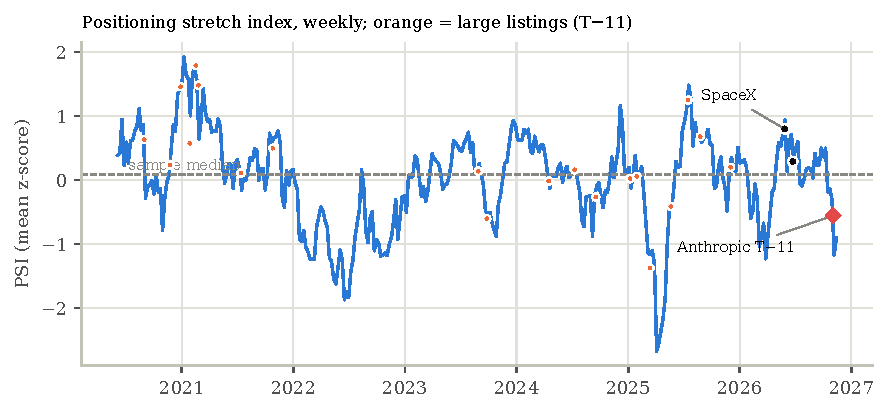
\includegraphics[width=\linewidth]{figures/f1_psi.pdf}
\caption{Positioning stretch index (weekly) and its value 11 sessions before each large listing. SpaceX listed near a local peak; Anthropic's T$-$11 reading is at the 20th percentile and its latest reading at the 12th.}\label{fig:psi}
\end{figure}

\section{Methodology}

\paragraph{State-matched placebo.} For each asset and window we split events by whether PSI at T$-$11 was above or below its sample median. We then compare each group's average move with random days drawn from the same PSI half. This separates an IPO effect from the ordinary behaviour of stretched or calm markets.

\paragraph{Panel regressions.} For every trading day $s$ from June 2020 to October 2026 we compute the return of asset $j$ over window $w$ starting at $s$, and estimate
\begin{equation}
r^{j,w}_{s} = \alpha + \beta\,\text{PSI}_s + \gamma\,E_s + \delta\,(E_s \times \text{PSI}_s) + \varepsilon_s,
\end{equation}
where $E_s=1$ if $s$ is a listing's T$-$11. The windows are T$-$10 to T$-$1 (pre), the listing day to T+5 (post), and T+6 to T+20 (late). $\delta$ measures how much more an asset moves around a large listing per unit of stretch, beyond what stretch alone predicts. Standard errors are Newey--West with lags equal to the window length \citep{newey1987}.

\paragraph{IPO cross-section.} For the 43 IPOs we relate PSI and each state variable at listing to the first-day return and to the return from the first close to day 63, raw and net of QQQ. We use Spearman correlations, OLS with HC3 errors controlling for the price revision and size, terciles, leave-one-year-out estimates and a year-block bootstrap that resamples listing years to allow for clustering in hot windows \citep{lowry2002}. Every family of tests is adjusted with Benjamini--Hochberg $q$-values \citep{benjamini1995}.

\section{Results}

\subsection{Baseline: what the unconditional data say}

Table~\ref{tab:recap} restates the companion note's main results. The median IPO is flat for a month and lower by month six, and it trails QQQ by about a third at day 126. Deals priced above their first range give back most. Across large listings there is no average pre-listing sell-off in Bitcoin or any other asset, and the soft week after listing does not survive multiple-testing correction.

\begin{table}[!htbp]\centering\footnotesize
\caption{Unconditional results from the companion note}\label{tab:recap}

\begin{threeparttable}
\begin{tabular}{lrc}
\toprule
Statistic & Estimate (\%) & 95\% CI or $p$ \\
\midrule
Median first-day return (43 IPOs) & +19.2 & -- \\
Median, day-1 close to day 63 & $-$7.0 & [$-$24, +8] \\
Median vs QQQ, day-1 close to day 126 & $-$33.8 & [$-$46, $-$15] \\
Above-range deals, median day 63 & $-$20.5 & [$-$28, $-$2] \\
Bitcoin, T$-$10 to T$-$1, 11 large listings & +3.6 & $p=0.67$ \\
S\&P 500, T+1 to T+5, 11 large listings & $-$1.2 & $p=0.03$ \\
\bottomrule
\end{tabular}
\begin{tablenotes}[flushleft]\footnotesize
\item \textit{Notes:} From \citet{frenzyfade2026}. Brackets: bootstrap 95\% CI of the median. Cross-asset $p$-values from permutation tests against random dates; none survives a correction for 56 tests.
\end{tablenotes}
\end{threeparttable}

\end{table}


\subsection{The market state before each large listing}

Table~\ref{tab:states} shows the state before every large listing. Stretched listings cluster in early 2021 (Affirm, Oscar Health, Coupang), mid-2025 (Figma) and June 2026 (SpaceX). Fifteen of the 22 listings came with PSI above its median, consistent with issuers timing deals into strong markets \citep{lowry2002}. SpaceX stands out on the momentum and crowding measures: high beta at the 92nd percentile, momentum crowding at the 98th, asset managers' E-mini length at the 92nd and a steep volatility curve (14th percentile of VIX/VIX3M).

\subsection{Does positioning condition the cross-asset response?}

The state-matched placebo (Table~\ref{tab:split}) gives little support to the deleveraging story. In the ten sessions before stretched listings, risk assets did not fall relative to other stretched days. If anything they rose: small caps $+2.1\%$ against $+0.4\%$ ($p=0.05$), the high-beta spread $+2.2\%$ against $+0.1\%$ ($p=0.05$), Bitcoin $+5.7\%$ against $+1.1\%$ ($p=0.13$). The soft week after listing appears mainly in \emph{calm} markets: the high-beta spread fell 2.3\% against a $+0.5\%$ placebo ($p=0.05$).

The panel regressions agree (Table~\ref{tab:reg}; Figure~\ref{fig:inter}). Of 27 interaction terms, one survives correction. It is positive: in stretched markets the high-beta spread gains an extra 2.5\% before large listings per unit of PSI ($t=3.1$, $q=0.05$). This is the frenzy feeding on itself, not a drain. Three negative interactions are significant before correction but not after: the Nasdaq-100 before listing ($-1.7\%$, $t=-2.3$) and gold before and after listing ($-1.7\%$ and $-2.5\%$, $t=-2.4$ and $-2.6$; $q=0.12$--$0.15$). They fit a ``sell what you can'' response in stretched markets, which is what SpaceX looked like, but the evidence is weak.

Individual state variables tell a similar story (Table~\ref{tab:varcorr}). A complacent volatility curve before a listing goes with weaker speculative growth stocks (VIX/VIX3M vs ARKK, $\rho=0.57$). Crowded momentum goes with weaker Bitcoin and ARKK ($\rho\approx-0.44$). More leveraged-fund length in E-mini futures goes with stronger Bitcoin ($\rho=0.56$). Each is plausible, but with 100 tests none has $q$ below 0.37.

\begin{table}[!htbp]\centering\footnotesize
\caption{Event windows split by positioning, against a state-matched placebo}\label{tab:split}
\resizebox{\linewidth}{!}{
\begin{threeparttable}
\begin{tabular}{lrrrrrrrr}
\toprule
& \multicolumn{4}{c}{T$-$10 to T$-$1} & \multicolumn{4}{c}{Listing day to T+5} \\ \cmidrule(lr){2-5}\cmidrule(lr){6-9} Asset & Stretched & Placebo & Not str. & Placebo & Stretched & Placebo & Not str. & Placebo \\
\midrule
S\&P 500 & +0.41 & +0.58 & +1.48 & +0.68 & $-$0.08 & +0.32 & $-$1.23 & +0.44 \\
Nasdaq 100 & $-$0.44 & +0.59 & +1.94 & +0.91 & $-$0.30 & +0.29 & $-$1.42 & +0.58 \\
Small caps & +2.09$^{*}$ & +0.36 & +0.84 & +0.58 & $-$0.32 & +0.13 & $-$1.80$^{*}$ & +0.44 \\
Spec. growth (ARKK) & +0.30 & $-$0.15 & +2.85 & +0.64 & $-$1.59 & $-$0.40 & $-$2.86 & +0.53 \\
Bitcoin & +5.74 & +1.12 & +0.96 & +1.40 & +2.57 & +0.05 & $-$0.32 & +1.52 \\
Gold & $-$0.20 & +0.59 & +1.54 & +0.47 & +0.13 & +0.32 & +0.88 & +0.36 \\
High beta - low vol & +2.16$^{*}$ & +0.14 & +0.89 & +0.94 & $-$0.70 & +0.06 & $-$2.29$^{*}$ & +0.53 \\
Momentum - market & $-$0.83 & $-$0.12 & +1.23 & +0.12 & $-$0.07 & $-$0.13 & $-$0.59 & +0.05 \\
Cross-asset momentum L/S & +1.11 & +1.46 & $-$3.80 & $-$0.51 & $-$0.25 & +0.53 & $-$0.32 & 0.00 \\
\bottomrule
\end{tabular}
\begin{tablenotes}[flushleft]\footnotesize
\item \textit{Notes:} Average log return in percent. Stretched = PSI at T$-$11 above its sample median (15 of 22 events). Placebo = average over all days in the same PSI half. Stars: permutation $p$ of the event average against 5,000 draws from the matched placebo days ($^{*}p<0.10$, $^{**}p<0.05$).
\end{tablenotes}
\end{threeparttable}
}
\end{table}

\begin{table}[!htbp]\centering\scriptsize
\caption{Panel regressions: does a large listing in a stretched market move assets more than a stretched day?}\label{tab:reg}
\resizebox{\linewidth}{!}{
\begin{threeparttable}
\begin{tabular}{llrrrrr}
\toprule
Asset & Window & PSI ($t$) & Event ($t$) & Event$\times$PSI ($t$) & $p$ & $q$ \\
\midrule
S\&P 500 & pre & $-$0.24 ($-$0.8) & 0.41 (0.9) & $-$0.55 ($-$1.2) & 0.23 & 0.49 \\
S\&P 500 & post & $-$0.10 ($-$0.5) & $-$1.50 ($-$1.7) & 1.99 (1.6) & 0.11 & 0.35 \\
S\&P 500 & late & $-$0.12 ($-$0.3) & 1.09 (1.2) & $-$0.07 ($-$0.1) & 0.95 & 0.95 \\
Nasdaq 100 & pre & $-$0.31 ($-$0.8) & 0.26 (0.4) & $-$1.65 ($-$2.3) & 0.022 & 0.15 \\
Nasdaq 100 & post & $-$0.23 ($-$0.9) & $-$1.83 ($-$1.7) & 2.34 (1.5) & 0.13 & 0.35 \\
Nasdaq 100 & late & $-$0.45 ($-$0.8) & 1.27 (1.1) & $-$0.11 ($-$0.1) & 0.94 & 0.95 \\
Small caps & pre & $-$0.46 ($-$1.3) & 1.30 (2.1) & 0.31 (0.4) & 0.71 & 0.91 \\
Small caps & post & $-$0.15 ($-$0.6) & $-$1.83 ($-$1.9) & 2.30 (1.8) & 0.069 & 0.35 \\
Small caps & late & $-$0.34 ($-$0.7) & 0.65 (0.6) & 0.30 (0.2) & 0.83 & 0.94 \\
Spec. growth (ARKK) & pre & $-$0.83 ($-$1.1) & 2.45 (2.4) & $-$3.56 ($-$1.6) & 0.11 & 0.35 \\
Spec. growth (ARKK) & post & $-$0.58 ($-$1.2) & $-$2.88 ($-$1.7) & 2.76 (1.1) & 0.29 & 0.56 \\
Spec. growth (ARKK) & late & $-$1.41 ($-$1.3) & 2.54 (1.0) & $-$1.38 ($-$0.5) & 0.60 & 0.85 \\
Bitcoin & pre & 0.36 (0.3) & 2.37 (1.1) & 1.18 (0.5) & 0.63 & 0.85 \\
Bitcoin & post & $-$0.08 ($-$0.1) & 0.27 (0.2) & 1.74 (0.9) & 0.39 & 0.66 \\
Bitcoin & late & 0.72 (0.4) & 5.86 (1.6) & $-$1.38 ($-$0.3) & 0.74 & 0.91 \\
Gold & pre & $-$0.17 ($-$0.5) & 0.48 (0.7) & $-$1.74 ($-$2.4) & 0.017 & 0.15 \\
Gold & post & $-$0.06 ($-$0.3) & 0.10 (0.2) & $-$0.10 ($-$0.2) & 0.87 & 0.94 \\
Gold & late & 0.28 (0.7) & 1.35 (1.5) & $-$2.53 ($-$2.6) & 0.009 & 0.12 \\
High beta - low vol & pre & $-$0.60 ($-$1.3) & 0.57 (0.8) & 2.53 (3.1) & 0.002 & 0.05 \\
High beta - low vol & post & $-$0.26 ($-$0.9) & $-$2.19 ($-$2.2) & 2.22 (1.7) & 0.089 & 0.35 \\
High beta - low vol & late & $-$0.57 ($-$0.8) & 0.64 (0.5) & $-$1.52 ($-$0.9) & 0.36 & 0.65 \\
Momentum - market & pre & $-$0.34 ($-$1.7) & 0.35 (0.7) & $-$1.15 ($-$1.4) & 0.17 & 0.39 \\
Momentum - market & post & $-$0.15 ($-$1.2) & $-$0.20 ($-$0.5) & 0.14 (0.2) & 0.85 & 0.94 \\
Momentum - market & late & $-$0.51 ($-$1.6) & 0.17 (0.3) & $-$0.60 ($-$0.6) & 0.54 & 0.85 \\
Cross-asset momentum L/S & pre & 2.00 (3.2) & $-$2.14 ($-$1.3) & 1.27 (0.5) & 0.62 & 0.85 \\
Cross-asset momentum L/S & post & 0.86 (1.7) & 0.02 (0.0) & $-$2.32 ($-$1.4) & 0.16 & 0.38 \\
Cross-asset momentum L/S & late & 1.43 (1.5) & $-$1.92 ($-$0.9) & 4.96 (1.5) & 0.12 & 0.35 \\
\bottomrule
\end{tabular}
\begin{tablenotes}[flushleft]\footnotesize
\item \textit{Notes:} Each row regresses the window return starting at every day $s$ (June 2020 to October 2026) on PSI$_s$, an event dummy (1 if $s$ is a listing's T$-$11) and their interaction. Coefficients in percent per unit of PSI (one PSI unit is about 1.5 standard deviations of the index); Newey--West $t$-statistics with lags equal to the window length. $q$: Benjamini--Hochberg across the 27 interaction tests.
\end{tablenotes}
\end{threeparttable}
}
\end{table}


\begin{figure}[!htbp]\centering
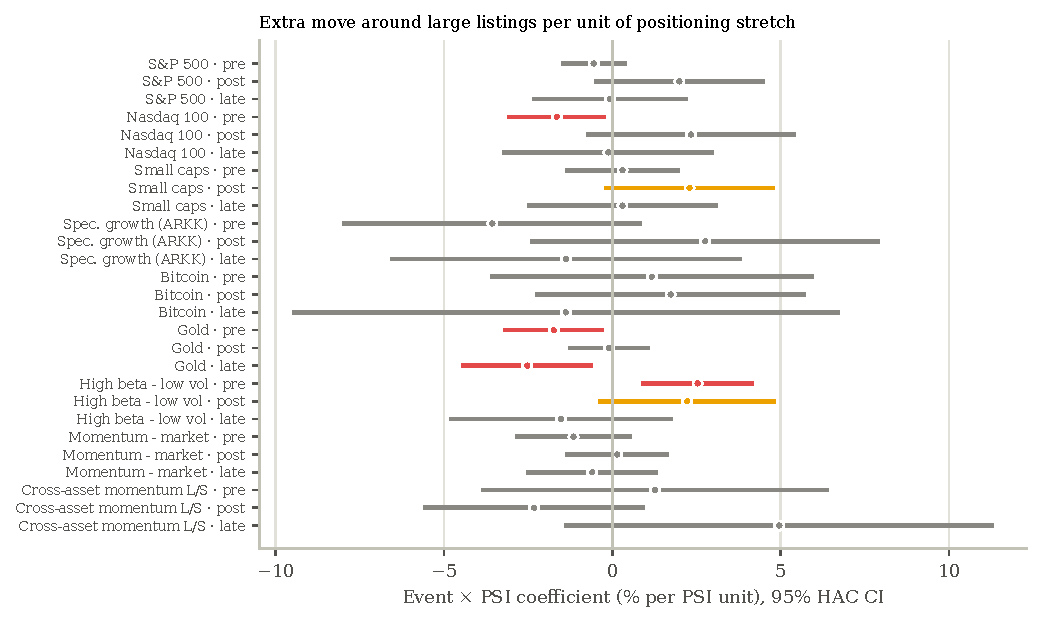
\includegraphics[width=0.92\linewidth]{figures/f4_inter.pdf}
\caption{Event$\times$PSI interaction coefficients with 95\% Newey--West confidence intervals. Red: $p<0.05$; amber: $p<0.10$.}\label{fig:inter}
\end{figure}

\begin{table}[!htbp]\centering\footnotesize
\caption{Which state variables line up with the event-window moves?}\label{tab:varcorr}

\begin{threeparttable}
\begin{tabular}{lllrrr}
\toprule
State at T$-$11 & Asset & Window & $\rho$ & $p$ & $q$ \\
\midrule
VIX / VIX3M & Spec. growth (ARKK) & pre & 0.57 & 0.005 & 0.37 \\
CFTC leveraged funds net / OI, E-mini & Bitcoin & pre & 0.56 & 0.007 & 0.37 \\
Bitcoin return, 63d & High beta - low vol & pre & 0.51 & 0.016 & 0.38 \\
CFTC leveraged funds net / OI, E-mini & High beta - low vol & pre & 0.50 & 0.017 & 0.38 \\
CFTC asset managers net / OI, E-mini & High beta - low vol & pre & $-$0.50 & 0.019 & 0.38 \\
Momentum vs market (MTUM/SPY), 63d & Spec. growth (ARKK) & pre & $-$0.44 & 0.038 & 0.57 \\
S\&P 500 return, 63d & Nasdaq 100 & pre & $-$0.44 & 0.042 & 0.57 \\
Momentum vs market (MTUM/SPY), 63d & Bitcoin & pre & $-$0.43 & 0.045 & 0.57 \\
High beta vs low vol (SPHB/SPLV), 63d & Cross-asset momentum L/S & pre & 0.41 & 0.057 & 0.62 \\
VIX / VIX3M & Nasdaq 100 & pre & 0.40 & 0.062 & 0.62 \\
Margin debt growth, YoY (Fed Z.1) & Bitcoin & pre & 0.39 & 0.077 & 0.65 \\
Bitcoin return, 63d & Cross-asset momentum L/S & pre & 0.37 & 0.095 & 0.65 \\
Momentum vs market (MTUM/SPY), 63d & Spec. growth (ARKK) & post & $-$0.36 & 0.098 & 0.65 \\
High beta vs low vol (SPHB/SPLV), 63d & High beta - low vol & pre & 0.36 & 0.099 & 0.65 \\
\bottomrule
\end{tabular}
\begin{tablenotes}[flushleft]\footnotesize
\item \textit{Notes:} Spearman correlation across the 22 large listings between the state variable and the event-window return. The 14 smallest $p$-values of 100 tests are shown; $q$ adjusts across all 100.
\end{tablenotes}
\end{threeparttable}

\end{table}


\subsection{Positioning and the IPO stock}

This is where positioning matters (Figure~\ref{fig:ipo}; Tables~\ref{tab:terciles}--\ref{tab:robust}). IPOs that list into a stretched market pop more and fade much harder. The rank correlation between PSI at listing and the day-63 return from the first close is $-0.51$ ($p<0.001$, $q=0.006$); net of QQQ it is $-0.44$ ($q=0.018$). The strongest single ingredient is the high-beta spread ($\rho=-0.52$, $q=0.006$). Bitcoin momentum ($-0.38$) and equity momentum (which predicts a bigger pop, $\rho=0.43$) also matter. Low realised volatility at listing goes with worse three-month returns, but only weakly ($\rho=0.28$, $p=0.07$). Futures positioning does not matter.

\begin{table}[!htbp]\centering\small
\caption{IPO outcomes by positioning at listing (PSI terciles)}\label{tab:terciles}

\begin{threeparttable}
\begin{tabular}{lrrrrrr}
\toprule
PSI tercile & $n$ & Median PSI & Pop & Day 21 & Day 63 & Day 63 vs QQQ \\
\midrule
Low PSI & 15 & $-$0.11 & +9 & +5 & +19 & +8 \\
Mid PSI & 14 & 0.16 & +29 & $-$2 & +4 & $-$3 \\
High PSI & 14 & 0.78 & +27 & $-$4 & $-$28 & $-$33 \\
\bottomrule
\end{tabular}
\begin{tablenotes}[flushleft]\footnotesize
\item \textit{Notes:} Medians in percent. PSI is the last weekly reading before listing. Returns after day 1 are measured from the first close.
\end{tablenotes}
\end{threeparttable}

\end{table}


\begin{figure}[!htbp]\centering
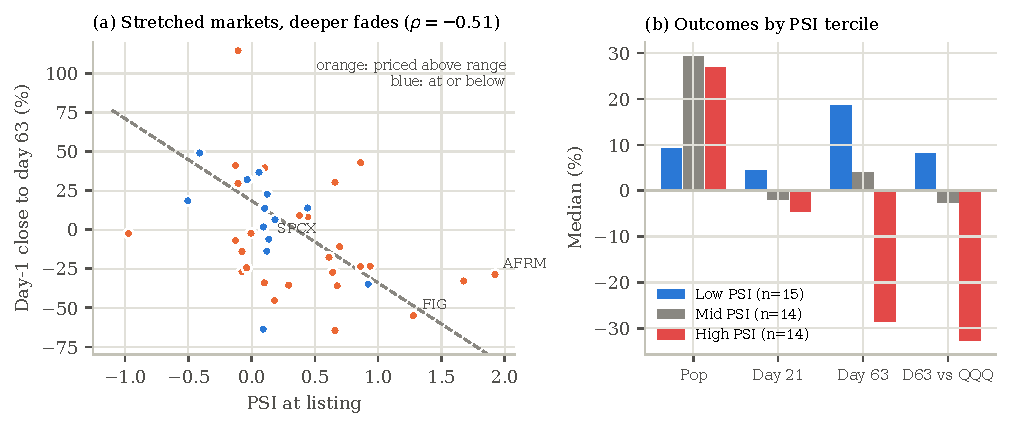
\includegraphics[width=\linewidth]{figures/f3_ipo.pdf}
\caption{(a) PSI at listing against the return from the first close to day 63, 43 IPOs. (b) Median outcomes by PSI tercile.}\label{fig:ipo}
\end{figure}

Two results separate positioning from demand. First, in a regression with the price revision and size (Table~\ref{tab:iporeg}), demand explains the pop and positioning explains the fade: the revision coefficient on the pop has $t=2.7$, while on the day-63 return only PSI is significant ($t=-2.0$). Second, the two-way split (Table~\ref{tab:2x2}) shows that a hot book is not enough to produce a deep fade. Above-range deals in stretched markets popped 35\% and then fell 28\%. Above-range deals in other markets popped about as much (32\%) but fell only 5\%.

\begin{table}[!htbp]\centering\footnotesize
\caption{Positioning at listing and IPO outcomes: rank correlations}\label{tab:ipocorr}

\begin{threeparttable}
\begin{tabular}{llrrr}
\toprule
State variable & Outcome & $\rho$ & $p$ & $q$ \\
\midrule
High beta vs low vol (SPHB/SPLV), 63d & Day 63 & $-$0.51 & $<$0.001 & 0.006 \\
Positioning stretch index (PSI) & Day 63 & $-$0.51 & $<$0.001 & 0.006 \\
High beta vs low vol (SPHB/SPLV), 63d & Day 63 vs QQQ & $-$0.48 & 0.001 & 0.009 \\
Positioning stretch index (PSI) & Day 63 vs QQQ & $-$0.44 & 0.003 & 0.018 \\
S\&P 500 return, 63d & Pop & 0.43 & 0.004 & 0.020 \\
Bitcoin return, 63d & Day 63 & $-$0.38 & 0.013 & 0.043 \\
Bitcoin return, 63d & Day 63 vs QQQ & $-$0.38 & 0.013 & 0.043 \\
Positioning stretch index (PSI) & Pop & 0.37 & 0.015 & 0.045 \\
Bitcoin return, 63d & Pop & 0.36 & 0.017 & 0.045 \\
High beta vs low vol (SPHB/SPLV), 63d & Pop & 0.34 & 0.026 & 0.063 \\
VIX / VIX3M & Pop & $-$0.30 & 0.054 & 0.117 \\
S\&P 500 realised vol, 21d & Day 63 & 0.28 & 0.069 & 0.137 \\
S\&P 500 return, 63d & Day 63 & $-$0.25 & 0.10 & 0.189 \\
S\&P 500 realised vol, 21d & Day 63 vs QQQ & 0.24 & 0.12 & 0.198 \\
\bottomrule
\end{tabular}
\begin{tablenotes}[flushleft]\footnotesize
\item \textit{Notes:} 43 IPOs. The 14 smallest $p$-values of 24 tests (8 state variables $\times$ 3 outcomes); $q$ adjusts across all 24.
\end{tablenotes}
\end{threeparttable}

\end{table}

\begin{table}[!htbp]\centering\footnotesize
\caption{Cross-sectional regressions: positioning versus demand}\label{tab:iporeg}

\begin{threeparttable}
\begin{tabular}{llrrrrr}
\toprule
Dependent variable & Spec. & PSI & Price revision & log market value & $R^2$ & $n$ \\
\midrule
First-day return & (1) & 0.36 (2.3) & -- & -- & 0.17 & 42 \\
 & (2) & 0.21 (1.3) & 1.01 (2.7) & 0.06 (1.0) & 0.30 & 42 \\
Day 63 return & (1) & $-$0.53 ($-$1.8) & -- & -- & 0.28 & 42 \\
 & (2) & $-$0.56 ($-$2.0) & 0.17 (0.3) & 0.06 (0.6) & 0.29 & 42 \\
Day 63 vs QQQ & (1) & $-$0.50 ($-$1.8) & -- & -- & 0.27 & 42 \\
 & (2) & $-$0.52 ($-$2.0) & 0.08 (0.1) & 0.07 (0.8) & 0.28 & 42 \\
\bottomrule
\end{tabular}
\begin{tablenotes}[flushleft]\footnotesize
\item \textit{Notes:} OLS with HC3 robust $t$-statistics in brackets. Returns as decimals. Price revision = offer vs midpoint of the first filed range. Demand drives the pop; positioning drives the fade.
\end{tablenotes}
\end{threeparttable}

\end{table}

\begin{table}[!htbp]\centering\footnotesize
\caption{Positioning and demand together}\label{tab:2x2}

\begin{threeparttable}
\begin{tabular}{lrrrrrr}
\toprule
& \multicolumn{3}{c}{Priced above first range} & \multicolumn{3}{c}{At or below range} \\ \cmidrule(lr){2-4}\cmidrule(lr){5-7} PSI at listing & $n$ & Pop & Day 63 & $n$ & Pop & Day 63 \\
\midrule
High PSI & 12 & +35 & $-$28 & 2 & +3 & $-$35 \\
Low or mid PSI & 16 & +32 & $-$5 & 12 & +4 & +16 \\
\bottomrule
\end{tabular}
\begin{tablenotes}[flushleft]\footnotesize
\item \textit{Notes:} Medians in percent. Day 63 measured from the first close.
\end{tablenotes}
\end{threeparttable}

\end{table}


The result is reasonably robust (Table~\ref{tab:robust}). It holds net of QQQ, without the 2021 listings ($\rho=-0.41$, $p=0.015$), and leaving out each listing year in turn ($\rho$ between $-0.41$ and $-0.55$). The weakest check is the year-block bootstrap, whose 95\% interval ($-0.59$ to $+0.03$) just touches zero. That is a reminder that stretched listings cluster in time, so the effective sample is smaller than 43.

\begin{table}[!htbp]\centering\footnotesize
\caption{Robustness of the PSI--fade relationship}\label{tab:robust}

\begin{threeparttable}
\begin{tabular}{lrrr}
\toprule
Test & $n$ & $\rho$ & $p$ \\
\midrule
Full sample, day 63 & 43 & $-$0.51 & $<$0.001 \\
Full sample, day 63 vs QQQ & 43 & $-$0.44 & 0.003 \\
Excluding 2021 listings, day 63 & 34 & $-$0.41 & 0.015 \\
Excluding 2021 listings, day 63 vs QQQ & 34 & $-$0.37 & 0.031 \\
Leave one listing year out, day 63 (range) & -- & $-$0.41 to $-$0.55 & -- \\
Year-block bootstrap 95\% CI, day 63 & -- & [$-$0.59, 0.03] & -- \\
Full sample, first-day return & 43 & 0.37 & 0.015 \\
PSI vs price revision & 42 & 0.35 & 0.021 \\
\bottomrule
\end{tabular}
\begin{tablenotes}[flushleft]\footnotesize
\item \textit{Notes:} Spearman correlations between PSI at listing and the outcome. The year-block bootstrap resamples listing years with replacement (5,000 draws), allowing for clustering of IPOs in hot windows.
\end{tablenotes}
\end{threeparttable}

\end{table}


\paragraph{Trading implications.} Conditioning on positioning makes the post-IPO fade a much better trade (Table~\ref{tab:strat}). Shorting every IPO from day 5 to day 63 earns 2.5\% on average with a CI that straddles zero. Shorting only those listed in the top PSI tercile earned 22\% on average (CI $+7\%$ to $+35\%$), worked 86\% of the time ($p_W=0.013$) and had a per-trade Sharpe ratio of 0.81. The same short on low-PSI listings lost 19\%. These figures are in-sample, because the terciles are drawn from the full-period PSI distribution, and they ignore borrow costs, which are high for new listings.

\begin{table}[!htbp]\centering\footnotesize
\caption{Positioning-conditioned strategies on the IPO stock}\label{tab:strat}
\resizebox{\linewidth}{!}{
\begin{threeparttable}
\begin{tabular}{lrrcrrrr}
\toprule
Strategy & $n$ & Mean & 95\% CI & Hit & $p_W$ & SR$_\text{trade}$ & SR$_\text{real}$ \\
\midrule
Short day 5 to 63, all IPOs & 43 & +2.5 & [$-$12, +15] & 65 & 0.17 & 0.06 & 0.15 \\
Short day 5 to 63, high-PSI tercile & 14 & +22.4 & [+7, +35] & 86 & 0.013 & 0.81 & 1.26 \\
Short day 5 to 63, low-PSI tercile & 15 & $-$18.8 & [$-$50, +7] & 40 & 0.30 & $-$0.32 & $-$0.51 \\
Long day 1 to 63, low-PSI tercile & 15 & +32.1 & [$-$2, +79] & 53 & 0.19 & 0.38 & 0.61 \\
Short day 5 to 63, high PSI and above range & 12 & +22.2 & [+5, +37] & 83 & 0.034 & 0.74 & 1.06 \\
\bottomrule
\end{tabular}
\begin{tablenotes}[flushleft]\footnotesize
\item \textit{Notes:} Percent per trade; shorts report the short-seller's return. SR$_\text{real}$ scales the per-trade Sharpe by the square root of the number of qualifying IPOs per year in the cohort (5.75 years). The tercile split uses the full-sample PSI distribution, so these are in-sample results; costs and borrow are ignored.
\end{tablenotes}
\end{threeparttable}
}
\end{table}


\section{SpaceX and Anthropic}

\paragraph{SpaceX listed into a stretched market.} Eleven sessions before its June listing, SpaceX met realised volatility at the 21st percentile and a steep volatility curve (VIX/VIX3M at the 14th). High beta was at the 92nd percentile, momentum crowding at the 98th and asset managers' E-mini length at the 92nd; PSI was at the 90th percentile (Table~\ref{tab:case}; Figure~\ref{fig:dash}). FINRA margin debt reached \$1.50tn at the end of June, its highest reading in the 13 months we have, and fell 5.6\% in July (Figure~\ref{fig:unwind}b). SpaceX's own path, a 19\% pop, a peak on day 3 and a return below the offer by day 23, is what the high-PSI tercile predicts.

\paragraph{Anthropic lists after an unwind.} When the S-1 became public on 26 October, the market was calm but not stretched: realised volatility at the 18th percentile, PSI at the 45th. Over the following three weeks the crowded trades unwound (Table~\ref{tab:moves}; Figure~\ref{fig:unwind}a). High beta lost 4.6\% relative to low volatility and momentum lost 2.3\% relative to the market. Bitcoin fell 12.5\% and MSTR 19.5\%. By 13 November momentum crowding was at its lowest reading since 2020, the high-beta spread at the 2nd percentile, realised volatility at the 85th and PSI at the 12th percentile. The sell-off before Anthropic therefore looks like a momentum unwind already under way, not a cash call by the IPO. Overall leverage has not come down: margin debt growth is at the 83rd percentile and asset managers' E-mini length at the 82nd.

\begin{table}[!htbp]\centering\footnotesize
\caption{SpaceX and Anthropic: the state of positioning}\label{tab:case}
\resizebox{\linewidth}{!}{
\begin{threeparttable}
\begin{tabular}{lrrrr}
\toprule
Variable & SpaceX, T$-$11 & ANT, S-1 public & ANT, T$-$11 & ANT, 13 Nov \\
\midrule
S\&P 500 realised vol, 21d & 10.2 (21) & 10.0 (18) & 11.3 (31) & 21.7 (85) \\
S\&P 500 return, 63d & +9.5 (80) & +3.3 (37) & $-$2.0 (18) & $-$2.4 (17) \\
VIX / VIX3M & 0.82 (14) & 0.92 (72) & 0.98 (92) & 0.94 (77) \\
High beta vs low vol (SPHB/SPLV), 63d & +24.2 (92) & +2.2 (47) & $-$8.7 (10) & $-$15.4 (2) \\
Momentum vs market (MTUM/SPY), 63d & +12.6 (98) & $-$2.5 (33) & $-$8.4 (6) & $-$13.6 (0) \\
Bitcoin return, 63d & +9.0 (51) & +25.3 (68) & +19.7 (61) & +5.8 (47) \\
CFTC leveraged funds net / OI, E-mini & $-$0.19 (19) & $-$0.19 (20) & $-$0.20 (14) & $-$0.19 (23) \\
CFTC asset managers net / OI, E-mini & 0.49 (92) & 0.47 (81) & 0.47 (85) & 0.47 (82) \\
Margin debt growth, YoY (Fed Z.1) & +30.5 (75) & +46.6 (83) & +46.6 (83) & +46.6 (83) \\
Positioning stretch index (PSI) & 0.80 (90) & 0.02 (45) & $-$0.56 (20) & $-$0.90 (12) \\
\bottomrule
\end{tabular}
\begin{tablenotes}[flushleft]\footnotesize
\item \textit{Notes:} Value (percentile rank since June 2020). SpaceX T$-$11 = 27 May 2026; Anthropic S-1 public = 26 October 2026; Anthropic T$-$11 = 3 November 2026.
\end{tablenotes}
\end{threeparttable}
}
\end{table}

\begin{table}[!htbp]\centering\footnotesize
\caption{The sell-offs: SpaceX pre-listing window and Anthropic so far}\label{tab:moves}

\begin{threeparttable}
\begin{tabular}{lrr}
\toprule
Asset & SpaceX, T$-$10 to T$-$1 & Anthropic, 3--13 Nov \\
\midrule
Bitcoin & $-$14.6 & $-$12.5 \\
MSTR & $-$23.3 & $-$19.5 \\
ARKK & $-$7.1 & $-$6.9 \\
Semis (SMH) & +1.6 & $-$6.3 \\
Nasdaq 100 & $-$2.5 & $-$0.8 \\
Gold & $-$6.6 & $-$1.1 \\
High beta $-$ low vol & $-$2.2 & $-$4.6 \\
Momentum $-$ market & +3.6 & $-$2.3 \\
\bottomrule
\end{tabular}
\begin{tablenotes}[flushleft]\footnotesize
\item \textit{Notes:} Log returns in percent. Anthropic's window covers 8 of its 10 pre-listing sessions.
\end{tablenotes}
\end{threeparttable}

\end{table}


\begin{figure}[!htbp]\centering
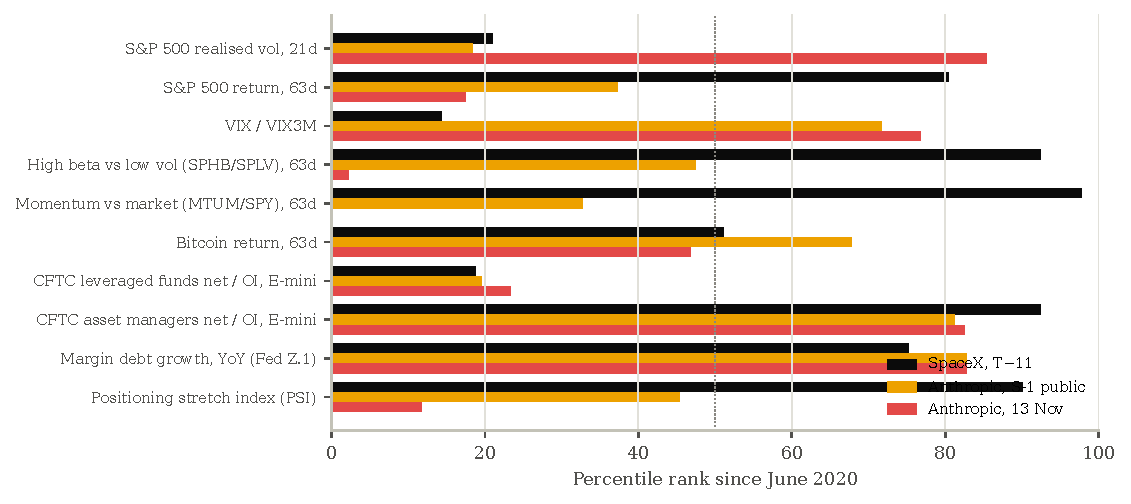
\includegraphics[width=0.92\linewidth]{figures/f2_dashboard.pdf}
\caption{Percentile rank of each state variable: SpaceX at T$-$11, Anthropic when its S-1 became public, and Anthropic on 13 November 2026.}\label{fig:dash}
\end{figure}

\begin{figure}[!htbp]\centering
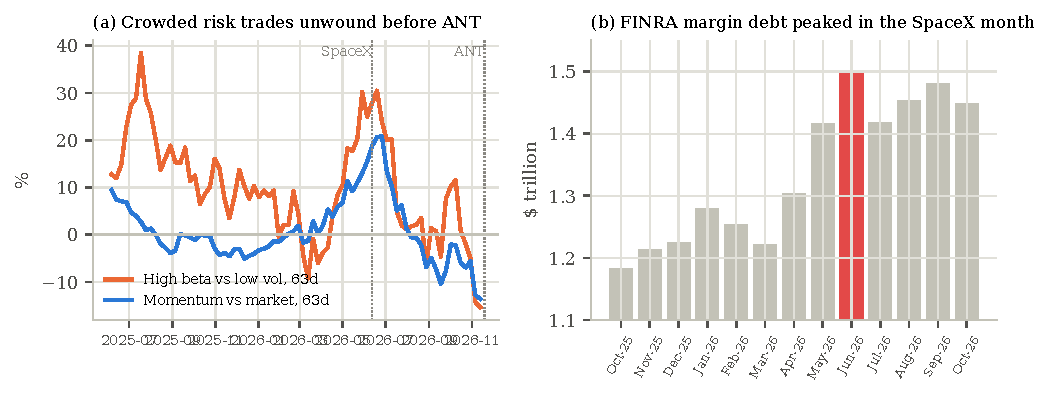
\includegraphics[width=\linewidth]{figures/f5_unwind.pdf}
\caption{(a) 63-day relative returns of high beta vs low volatility and of momentum vs the market. (b) FINRA debit balances in customers' margin accounts, October 2025 to October 2026.}\label{fig:unwind}
\end{figure}

\paragraph{What this implies.} The cohort's low-PSI listings popped 9\% (median) and were up 19\% from their first close by day 63; the high-PSI listings popped 27\% and fell 28\%. If Anthropic prices above its \$70--78 range, demand points to a large pop, and Table~\ref{tab:2x2} suggests that in a non-stretched market such deals gave back far less than in stretched ones. Two qualifications matter. Anthropic is far larger than any low-PSI listing in the sample. And leverage is still high, so a further unwind in the broader market remains possible, independent of the IPO. We would update the conditional plan of the companion note as follows: the fade from day 5 is a weaker trade than SpaceX suggests, unless PSI recovers sharply into and after the listing, which would reopen the stretched-market playbook.

\section{Limitations}

\begin{itemize}
\item \textbf{Small, clustered samples.} 22 events and 43 IPOs, with stretched listings concentrated in 2021 and 2025--26. The year-block bootstrap, which respects this clustering, gives an interval that just includes zero ($-0.59$ to $+0.03$).
\item \textbf{Index construction.} PSI equally weights five standardised variables, and the standardisation uses the full sample (a mild look-ahead in levels, not in ranks within a year). Other weights or variables could give different results; we report the components separately for this reason.
\item \textbf{Leverage data.} CFTC leveraged-fund positions mix directional bets with basis trades; Z.1 margin data are quarterly and lagged; FINRA monthly data were available only for the last 13 months. Direct measures of prime-brokerage leverage, systematic-fund exposure and options positioning were not available.
\item \textbf{In-sample strategies.} Tercile strategies use full-sample breakpoints and ignore borrow costs and the delayed listing of options.
\end{itemize}

\section{Conclusion}

The SpaceX pattern, a sell-off in crowded risk assets before a mega-IPO, does not generalise across large listings, and conditioning on positioning does not rescue it: if anything, stretched markets chase high beta into large deals. Positioning does explain something important, though: how far the IPO stock itself rises and falls. In stretched markets IPOs pop more and give much more back; in calm or de-risked markets the fade largely disappears. SpaceX listed at the top of the positioning cycle. Anthropic lists after the crowded trades have already unwound, which argues for a smaller pop and a shallower fade than SpaceX, provided that the remaining leverage does not unwind as well.

\vspace{1em}
\noindent{\footnotesize\textit{Disclaimer.} This note is for research and discussion. It is not investment advice or a recommendation to buy or sell any security. Anthropic figures are based on public filings and press reports as of 15 November 2026.}

\bibliographystyle{plainnat}
\bibliography{refs}

\clearpage
\appendix
\section{Appendix}
\begin{table*}[!htbp]\centering\scriptsize
\caption{Market state before each large listing (percentile ranks)}\label{tab:states}
\resizebox{\linewidth}{!}{
\begin{threeparttable}
\begin{tabular}{llrrrrrrrrrrr}
\toprule
Listed & Company & \$bn & RV21 & Mom63 & VIX/3M & $\beta$ spread & MTUM & BTC & Lev.\ funds & Margin & PSI & PSI pct \\
\midrule
2020-09-16 & Snowflake + Unity & 4.66 & 5 & 94 & 17 & 44 & 90 & 64 & 53 & 23 & 0.63 & 83 \\
2020-12-09 & DoorDash + Airbnb & 6.86 & 88 & 41 & 56 & 90 & 37 & 89 & 88 & 56 & 0.24 & 62 \\
2021-01-13 & Affirm & 1.21 & 9 & 89 & 39 & 95 & 41 & 97 & 88 & 56 & 1.46 & 98 \\
2021-02-11 & Bumble & 2.15 & 59 & 85 & 98 & 93 & 54 & 96 & 79 & 79 & 0.57 & 80 \\
2021-03-03 & Oscar Health & 1.42 & 65 & 88 & 1 & 97 & 89 & 99 & 76 & 79 & 1.79 & 100 \\
2021-03-11 & Coupang & 4.55 & 64 & 85 & 15 & 97 & 57 & 98 & 69 & 79 & 1.48 & 98 \\
2021-07-29 & Robinhood & 2.09 & 17 & 60 & 3 & 27 & 13 & 1 & 83 & 96 & 0.11 & 52 \\
2021-11-10 & Rivian & 11.93 & 53 & 42 & 4 & 61 & 83 & 84 & 92 & 88 & 0.50 & 76 \\
2023-09-14 & Arm & 4.87 & 44 & 65 & 45 & 57 & 59 & 41 & 44 & 8 & 0.14 & 54 \\
2023-10-11 & Birkenstock & 1.48 & 41 & 17 & 86 & 25 & 53 & 24 & 43 & 8 & $-$0.60 & 19 \\
2024-05-01 & Viking & 1.54 & 36 & 59 & 91 & 50 & 91 & 82 & 36 & 48 & $-$0.01 & 43 \\
2024-07-25 & Lineage & 4.44 & 0 & 73 & 53 & 36 & 53 & 21 & 52 & 52 & 0.16 & 56 \\
2024-10-02 & StandardAero & 1.44 & 54 & 35 & 47 & 14 & 28 & 32 & 67 & 52 & $-$0.26 & 29 \\
2025-01-24 & Venture Global & 1.75 & 62 & 40 & 74 & 55 & 48 & 86 & 39 & 44 & 0.02 & 45 \\
2025-02-13 & SailPoint & 1.38 & 59 & 42 & 67 & 47 & 63 & 86 & 21 & 60 & 0.06 & 48 \\
2025-03-28 & CoreWeave & 1.5 & 72 & 4 & 98 & 2 & 64 & 21 & 58 & 60 & $-$1.37 & 4 \\
2025-06-05 & Circle & 1.05 & 65 & 15 & 46 & 14 & 81 & 53 & 52 & 31 & $-$0.41 & 24 \\
2025-07-31 & Figma & 1.22 & 10 & 97 & 33 & 98 & 81 & 78 & 27 & 40 & 1.25 & 96 \\
2025-09-10 & Klarna + Figure + Gemini & 2.58 & 36 & 87 & 13 & 87 & 28 & 44 & 25 & 40 & 0.68 & 85 \\
2025-12-17 & Medline & 6.27 & 59 & 58 & 21 & 76 & 28 & 19 & 25 & 64 & 0.20 & 58 \\
2026-06-12 & SpaceX & 75 & 21 & 80 & 14 & 92 & 98 & 51 & 19 & 75 & 0.80 & 90 \\
2026-07-10 & SK hynix ADR & 26.5 & 69 & 92 & 68 & 92 & 99 & 25 & 16 & 75 & 0.29 & 65 \\
\midrule
-- & Anthropic, T-11 (3 Nov 2026) & -- & 31 & 18 & 92 & 10 & 6 & 61 & 14 & 83 & $-$0.56 & 20 \\
-- & Latest (13 Nov 2026) & -- & 85 & 17 & 77 & 2 & 0 & 47 & 23 & 83 & $-$0.90 & 12 \\
-- & Anthropic S-1 public (26 Oct 2026) & -- & 18 & 37 & 72 & 47 & 33 & 68 & 20 & 83 & 0.02 & 45 \\
\bottomrule
\end{tabular}
\begin{tablenotes}[flushleft]\footnotesize
\item \textit{Notes:} Percentile ranks (0--100) of each state variable against all days June 2020 to November 2026, measured at T$-$11 (the close before the pre-listing window). Low RV21 and low VIX/VIX3M are the stretched readings for those columns. Anthropic's T$-$11 is 3 November 2026; its S-1 became public on 26 October.
\end{tablenotes}
\end{threeparttable}
}
\end{table*}


\end{document}
